%Universal diagram
\begin{figure}[ht!]
\centering
\scalebox{0.65}{
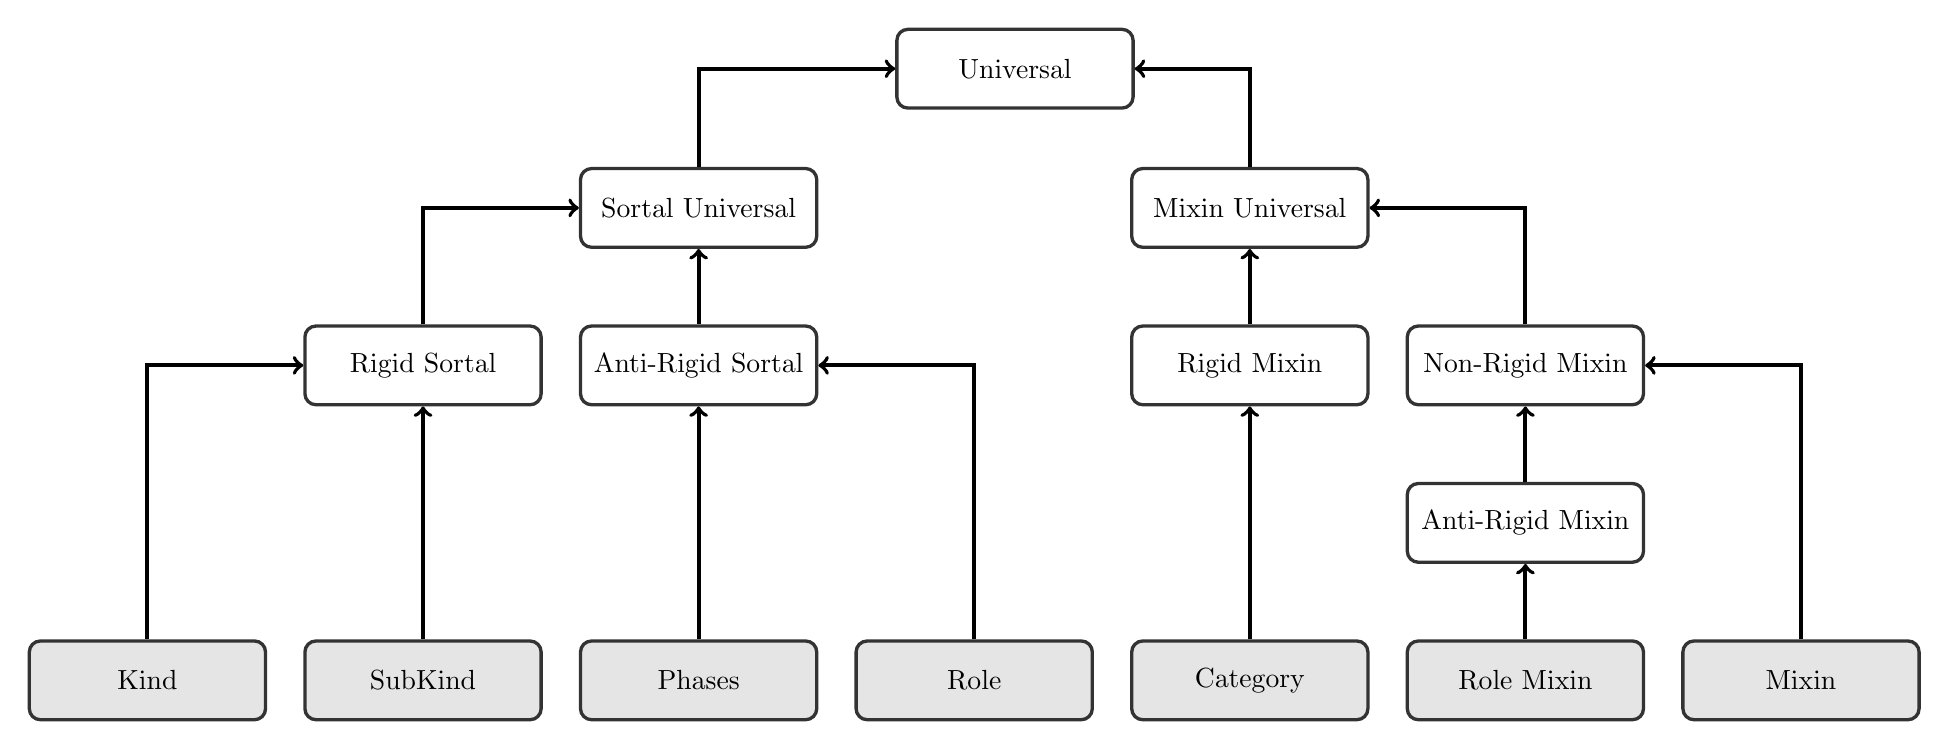
\begin{tikzpicture}[squarednode/.style={rectangle, 
					rounded corners, 
					very thick,
 					minimum width=3cm,
					minimum height=1cm,
					draw=black!80, 
					fill=white!10},
					squarednode2/.style={rectangle, 
					rounded corners, 
					very thick,
 					minimum width=3cm,
					minimum height=1cm,
					draw=black!80, 
					fill=black!10},
					node distance = 2.5cm
					]
					


%top node
\node[squarednode]  (Univ) {Universal};

%second level
\node[squarednode]  (Sortal) [below left of = Univ, xshift=-2.25cm] {Sortal Universal};
\node[squarednode]  (Mixin) [right of = Sortal, node distance = 7cm] {Mixin Universal};

% third level
\node[squarednode]  (ARigidSor) [below of = Sortal, node distance = 2cm] {Anti-Rigid Sortal};
\node[squarednode]  (RigidSor) [left of = ARigidSor, node distance = 3.5cm] {Rigid Sortal};

\node[squarednode]  (RigidMix) [below of = Mixin, node distance = 2cm] {Rigid Mixin};
\node[squarednode]  (NRigidMix) [right of = RigidMix, node distance = 3.5cm] {Non-Rigid Mixin};
\node[squarednode]  (ARigidMix) [below of = NRigidMix, node distance = 2cm] {Anti-Rigid Mixin};

% leaves
\node[squarednode2]  (SubKind) [below of = RigidSor, node distance = 4cm] {SubKind};
\node[squarednode2]  (Kind) [left of= SubKind, node distance = 3.5cm] {Kind};


\node[squarednode2]  (RoleMix) [below of = ARigidMix, node distance = 2cm] {Role Mixin};
\node[squarednode2]  (MixinL) [right of= RoleMix, node distance = 3.5cm] {Mixin};

\node[squarednode2]  (Cat) [below of = RigidMix, node distance = 4cm] {Category};

\node[squarednode2]  (Phases) [below of = ARigidSor, node distance = 4cm] {Phases};
\node[squarednode2]  (Role) [right of=Phases, node distance = 3.5cm] {Role};



% Arrows 
\draw [->, line width=0.5mm] (Sortal.north) |- (Univ.west);
\draw [->, line width=0.5mm] (Mixin.north) |- (Univ.east);

\draw [->, line width=0.5mm] (RigidSor.north) |- (Sortal.west);
\draw [->, line width=0.5mm] (ARigidSor.north) -- (Sortal.south);
\draw [->, line width=0.5mm] (NRigidMix.north) |- (Mixin.east);
\draw [->, line width=0.5mm] (RigidMix.north) -- (Mixin.south);
\draw [->, line width=0.5mm] (ARigidMix.north) -- (NRigidMix.south);

\draw [->, line width=0.5mm] (Kind.north) |- (RigidSor.west);
\draw [->, line width=0.5mm] (SubKind.north) -- (RigidSor.south);
\draw [->, line width=0.5mm] (Phases.north) -- (ARigidSor.south);
\draw [->, line width=0.5mm] (Role.north) |- (ARigidSor.east);
\draw [->, line width=0.5mm] (Cat.north) -- (RigidMix.south);
\draw [->, line width=0.5mm] (RoleMix.north) -- (ARigidMix.south);
\draw [->, line width=0.5mm] (MixinL.north) |- (NRigidMix.east);

\end{tikzpicture}
}%endscale
\caption{Universal classification Diagram \citep{guizzardi_ontological_2005}}
\label{fig:Univ_diag}
\end{figure}